% Created by tikzDevice version 0.10.1 on 2020-02-15 16:08:33
% !TEX encoding = UTF-8 Unicode
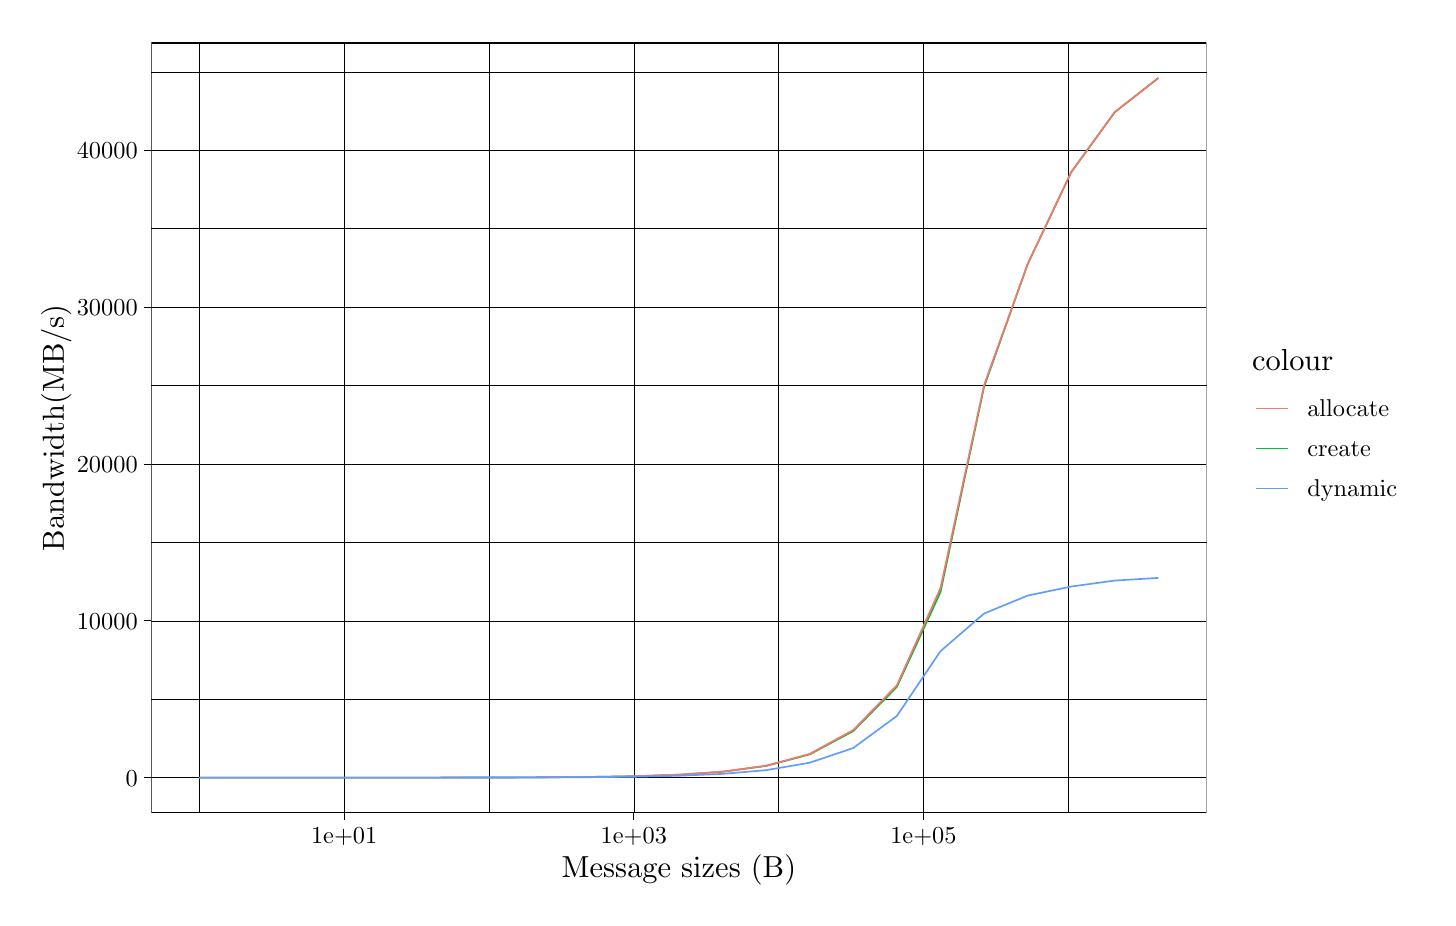
\begin{tikzpicture}[x=1pt,y=1pt]
\definecolor{fillColor}{RGB}{255,255,255}
\path[use as bounding box,fill=fillColor,fill opacity=0.00] (0,0) rectangle (505.89,314.37);
\begin{scope}
\path[clip] (  0.00,  0.00) rectangle (505.89,314.37);
\definecolor{drawColor}{RGB}{255,255,255}
\definecolor{fillColor}{RGB}{255,255,255}

\path[draw=drawColor,line width= 0.6pt,line join=round,line cap=round,fill=fillColor] (  0.00,  0.00) rectangle (505.89,314.37);
\end{scope}
\begin{scope}
\path[clip] ( 44.71, 30.72) rectangle (425.93,308.87);
\definecolor{fillColor}{RGB}{255,255,255}

\path[fill=fillColor] ( 44.71, 30.72) rectangle (425.93,308.87);
\definecolor{drawColor}{RGB}{0,0,0}

\path[draw=drawColor,line width= 0.0pt,line join=round] ( 44.71, 71.70) --
	(425.93, 71.70);

\path[draw=drawColor,line width= 0.0pt,line join=round] ( 44.71,128.35) --
	(425.93,128.35);

\path[draw=drawColor,line width= 0.0pt,line join=round] ( 44.71,185.01) --
	(425.93,185.01);

\path[draw=drawColor,line width= 0.0pt,line join=round] ( 44.71,241.67) --
	(425.93,241.67);

\path[draw=drawColor,line width= 0.0pt,line join=round] ( 44.71,298.32) --
	(425.93,298.32);

\path[draw=drawColor,line width= 0.0pt,line join=round] ( 62.04, 30.72) --
	( 62.04,308.87);

\path[draw=drawColor,line width= 0.0pt,line join=round] (166.70, 30.72) --
	(166.70,308.87);

\path[draw=drawColor,line width= 0.0pt,line join=round] (271.36, 30.72) --
	(271.36,308.87);

\path[draw=drawColor,line width= 0.0pt,line join=round] (376.02, 30.72) --
	(376.02,308.87);

\path[draw=drawColor,line width= 0.1pt,line join=round] ( 44.71, 43.37) --
	(425.93, 43.37);

\path[draw=drawColor,line width= 0.1pt,line join=round] ( 44.71,100.02) --
	(425.93,100.02);

\path[draw=drawColor,line width= 0.1pt,line join=round] ( 44.71,156.68) --
	(425.93,156.68);

\path[draw=drawColor,line width= 0.1pt,line join=round] ( 44.71,213.34) --
	(425.93,213.34);

\path[draw=drawColor,line width= 0.1pt,line join=round] ( 44.71,269.99) --
	(425.93,269.99);

\path[draw=drawColor,line width= 0.1pt,line join=round] (114.37, 30.72) --
	(114.37,308.87);

\path[draw=drawColor,line width= 0.1pt,line join=round] (219.03, 30.72) --
	(219.03,308.87);

\path[draw=drawColor,line width= 0.1pt,line join=round] (323.69, 30.72) --
	(323.69,308.87);
\definecolor{drawColor}{RGB}{0,186,56}

\path[draw=drawColor,line width= 0.6pt,line join=round] ( 62.04, 43.37) --
	( 77.80, 43.37) --
	( 93.55, 43.37) --
	(109.30, 43.37) --
	(125.05, 43.38) --
	(140.81, 43.38) --
	(156.56, 43.40) --
	(172.31, 43.43) --
	(188.07, 43.50) --
	(203.82, 43.63) --
	(219.57, 43.89) --
	(235.32, 44.42) --
	(251.08, 45.49) --
	(266.83, 47.59) --
	(282.58, 51.77) --
	(298.33, 60.20) --
	(314.09, 76.18) --
	(329.84,110.42) --
	(345.59,184.59) --
	(361.35,228.94) --
	(377.10,262.16) --
	(392.85,283.85) --
	(408.60,296.20);
\definecolor{drawColor}{RGB}{248,118,109}

\path[draw=drawColor,line width= 0.6pt,line join=round] ( 62.04, 43.37) --
	( 77.80, 43.37) --
	( 93.55, 43.37) --
	(109.30, 43.37) --
	(125.05, 43.38) --
	(140.81, 43.38) --
	(156.56, 43.40) --
	(172.31, 43.43) --
	(188.07, 43.50) --
	(203.82, 43.64) --
	(219.57, 43.90) --
	(235.32, 44.45) --
	(251.08, 45.53) --
	(266.83, 47.69) --
	(282.58, 51.94) --
	(298.33, 60.58) --
	(314.09, 76.74) --
	(329.84,111.87) --
	(345.59,185.19) --
	(361.35,229.02) --
	(377.10,262.25) --
	(392.85,283.92) --
	(408.60,296.23);
\definecolor{drawColor}{RGB}{97,156,255}

\path[draw=drawColor,line width= 0.6pt,line join=round] ( 62.04, 43.37) --
	( 77.80, 43.37) --
	( 93.55, 43.37) --
	(109.30, 43.37) --
	(125.05, 43.37) --
	(140.81, 43.38) --
	(156.56, 43.39) --
	(172.31, 43.41) --
	(188.07, 43.45) --
	(203.82, 43.54) --
	(219.57, 43.71) --
	(235.32, 44.05) --
	(251.08, 44.73) --
	(266.83, 46.07) --
	(282.58, 48.76) --
	(298.33, 54.08) --
	(314.09, 65.66) --
	(329.84, 89.07) --
	(345.59,102.67) --
	(361.35,109.15) --
	(377.10,112.43) --
	(392.85,114.58) --
	(408.60,115.55);
\definecolor{drawColor}{RGB}{0,0,0}

\path[draw=drawColor,line width= 0.6pt,line join=round,line cap=round] ( 44.71, 30.72) rectangle (425.93,308.87);
\end{scope}
\begin{scope}
\path[clip] (  0.00,  0.00) rectangle (505.89,314.37);
\definecolor{drawColor}{RGB}{0,0,0}

\node[text=drawColor,anchor=base east,inner sep=0pt, outer sep=0pt, scale=  0.88] at ( 39.76, 40.34) {0};

\node[text=drawColor,anchor=base east,inner sep=0pt, outer sep=0pt, scale=  0.88] at ( 39.76, 96.99) {10000};

\node[text=drawColor,anchor=base east,inner sep=0pt, outer sep=0pt, scale=  0.88] at ( 39.76,153.65) {20000};

\node[text=drawColor,anchor=base east,inner sep=0pt, outer sep=0pt, scale=  0.88] at ( 39.76,210.31) {30000};

\node[text=drawColor,anchor=base east,inner sep=0pt, outer sep=0pt, scale=  0.88] at ( 39.76,266.96) {40000};
\end{scope}
\begin{scope}
\path[clip] (  0.00,  0.00) rectangle (505.89,314.37);
\definecolor{drawColor}{RGB}{0,0,0}

\path[draw=drawColor,line width= 0.3pt,line join=round] ( 41.96, 43.37) --
	( 44.71, 43.37);

\path[draw=drawColor,line width= 0.3pt,line join=round] ( 41.96,100.02) --
	( 44.71,100.02);

\path[draw=drawColor,line width= 0.3pt,line join=round] ( 41.96,156.68) --
	( 44.71,156.68);

\path[draw=drawColor,line width= 0.3pt,line join=round] ( 41.96,213.34) --
	( 44.71,213.34);

\path[draw=drawColor,line width= 0.3pt,line join=round] ( 41.96,269.99) --
	( 44.71,269.99);
\end{scope}
\begin{scope}
\path[clip] (  0.00,  0.00) rectangle (505.89,314.37);
\definecolor{drawColor}{RGB}{0,0,0}

\path[draw=drawColor,line width= 0.3pt,line join=round] (114.37, 27.97) --
	(114.37, 30.72);

\path[draw=drawColor,line width= 0.3pt,line join=round] (219.03, 27.97) --
	(219.03, 30.72);

\path[draw=drawColor,line width= 0.3pt,line join=round] (323.69, 27.97) --
	(323.69, 30.72);
\end{scope}
\begin{scope}
\path[clip] (  0.00,  0.00) rectangle (505.89,314.37);
\definecolor{drawColor}{RGB}{0,0,0}

\node[text=drawColor,anchor=base,inner sep=0pt, outer sep=0pt, scale=  0.88] at (114.37, 19.71) {1e+01};

\node[text=drawColor,anchor=base,inner sep=0pt, outer sep=0pt, scale=  0.88] at (219.03, 19.71) {1e+03};

\node[text=drawColor,anchor=base,inner sep=0pt, outer sep=0pt, scale=  0.88] at (323.69, 19.71) {1e+05};
\end{scope}
\begin{scope}
\path[clip] (  0.00,  0.00) rectangle (505.89,314.37);
\definecolor{drawColor}{RGB}{0,0,0}

\node[text=drawColor,anchor=base,inner sep=0pt, outer sep=0pt, scale=  1.10] at (235.32,  7.44) {Message sizes (B)};
\end{scope}
\begin{scope}
\path[clip] (  0.00,  0.00) rectangle (505.89,314.37);
\definecolor{drawColor}{RGB}{0,0,0}

\node[text=drawColor,rotate= 90.00,anchor=base,inner sep=0pt, outer sep=0pt, scale=  1.10] at ( 13.08,169.80) {Bandwidth(MB/s)};
\end{scope}
\begin{scope}
\path[clip] (  0.00,  0.00) rectangle (505.89,314.37);
\definecolor{fillColor}{RGB}{255,255,255}

\path[fill=fillColor] (436.93,135.11) rectangle (500.39,204.49);
\end{scope}
\begin{scope}
\path[clip] (  0.00,  0.00) rectangle (505.89,314.37);
\definecolor{drawColor}{RGB}{0,0,0}

\node[text=drawColor,anchor=base west,inner sep=0pt, outer sep=0pt, scale=  1.10] at (442.43,190.44) {colour};
\end{scope}
\begin{scope}
\path[clip] (  0.00,  0.00) rectangle (505.89,314.37);
\definecolor{fillColor}{RGB}{255,255,255}

\path[fill=fillColor] (442.43,169.52) rectangle (456.89,183.97);
\end{scope}
\begin{scope}
\path[clip] (  0.00,  0.00) rectangle (505.89,314.37);
\definecolor{drawColor}{RGB}{248,118,109}

\path[draw=drawColor,line width= 0.6pt,line join=round] (443.88,176.74) -- (455.44,176.74);
\end{scope}
\begin{scope}
\path[clip] (  0.00,  0.00) rectangle (505.89,314.37);
\definecolor{drawColor}{RGB}{248,118,109}

\path[draw=drawColor,line width= 0.6pt,line join=round] (443.88,176.74) -- (455.44,176.74);
\end{scope}
\begin{scope}
\path[clip] (  0.00,  0.00) rectangle (505.89,314.37);
\definecolor{drawColor}{RGB}{248,118,109}

\path[draw=drawColor,line width= 0.6pt,line join=round] (443.88,176.74) -- (455.44,176.74);
\end{scope}
\begin{scope}
\path[clip] (  0.00,  0.00) rectangle (505.89,314.37);
\definecolor{fillColor}{RGB}{255,255,255}

\path[fill=fillColor] (442.43,155.06) rectangle (456.89,169.52);
\end{scope}
\begin{scope}
\path[clip] (  0.00,  0.00) rectangle (505.89,314.37);
\definecolor{drawColor}{RGB}{0,186,56}

\path[draw=drawColor,line width= 0.6pt,line join=round] (443.88,162.29) -- (455.44,162.29);
\end{scope}
\begin{scope}
\path[clip] (  0.00,  0.00) rectangle (505.89,314.37);
\definecolor{drawColor}{RGB}{0,186,56}

\path[draw=drawColor,line width= 0.6pt,line join=round] (443.88,162.29) -- (455.44,162.29);
\end{scope}
\begin{scope}
\path[clip] (  0.00,  0.00) rectangle (505.89,314.37);
\definecolor{drawColor}{RGB}{0,186,56}

\path[draw=drawColor,line width= 0.6pt,line join=round] (443.88,162.29) -- (455.44,162.29);
\end{scope}
\begin{scope}
\path[clip] (  0.00,  0.00) rectangle (505.89,314.37);
\definecolor{fillColor}{RGB}{255,255,255}

\path[fill=fillColor] (442.43,140.61) rectangle (456.89,155.06);
\end{scope}
\begin{scope}
\path[clip] (  0.00,  0.00) rectangle (505.89,314.37);
\definecolor{drawColor}{RGB}{97,156,255}

\path[draw=drawColor,line width= 0.6pt,line join=round] (443.88,147.84) -- (455.44,147.84);
\end{scope}
\begin{scope}
\path[clip] (  0.00,  0.00) rectangle (505.89,314.37);
\definecolor{drawColor}{RGB}{97,156,255}

\path[draw=drawColor,line width= 0.6pt,line join=round] (443.88,147.84) -- (455.44,147.84);
\end{scope}
\begin{scope}
\path[clip] (  0.00,  0.00) rectangle (505.89,314.37);
\definecolor{drawColor}{RGB}{97,156,255}

\path[draw=drawColor,line width= 0.6pt,line join=round] (443.88,147.84) -- (455.44,147.84);
\end{scope}
\begin{scope}
\path[clip] (  0.00,  0.00) rectangle (505.89,314.37);
\definecolor{drawColor}{RGB}{0,0,0}

\node[text=drawColor,anchor=base west,inner sep=0pt, outer sep=0pt, scale=  0.88] at (462.39,173.71) {allocate};
\end{scope}
\begin{scope}
\path[clip] (  0.00,  0.00) rectangle (505.89,314.37);
\definecolor{drawColor}{RGB}{0,0,0}

\node[text=drawColor,anchor=base west,inner sep=0pt, outer sep=0pt, scale=  0.88] at (462.39,159.26) {create};
\end{scope}
\begin{scope}
\path[clip] (  0.00,  0.00) rectangle (505.89,314.37);
\definecolor{drawColor}{RGB}{0,0,0}

\node[text=drawColor,anchor=base west,inner sep=0pt, outer sep=0pt, scale=  0.88] at (462.39,144.81) {dynamic};
\end{scope}
\end{tikzpicture}
